\section{眼睛中图像的形成}
\subsection{角膜的折射}
\begin{frame}
    \frametitle{眼睛中图像的形成}

    眼睛接收环境中由物体发射或反射的光线,并将他们聚焦于视网膜以成像,如图\ref{pic3-1}。光在穿过角膜弯曲的表面时候
    会发生偏折。自折射表面至平行光的汇聚点的距离称为\textbf{焦距}焦距和角膜的曲率有关:弯曲程度越高,焦距越短。
    焦距的倒数称为\textbf{屈光度}(diopter)。角膜的折射力约42屈光度。
    \begin{figure}
        \centering
        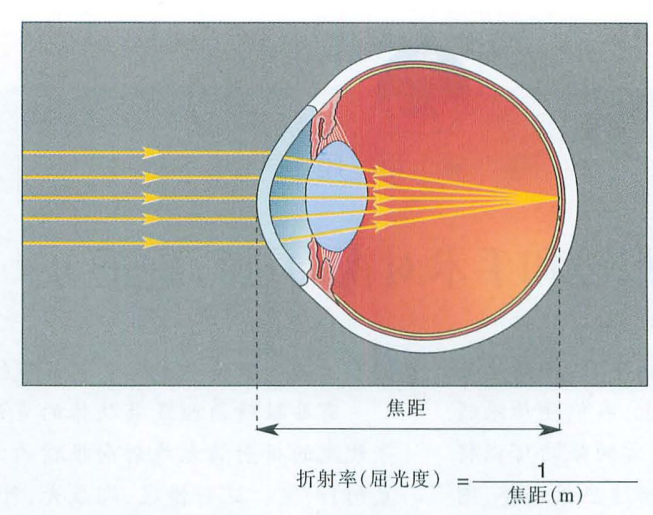
\includegraphics[height=0.3\textwidth]{img/pic3-1.png}
        \caption{角膜的折射作用\label{pic3-1}}
        % [width=0.8\textwidth,height=0.5\textwidth]
    \end{figure}

\end{frame}
\subsection{晶状体的适应性调节}
\subsection{瞳孔对光反射}

\begin{frame}
    \frametitle{晶状体与瞳孔的调节作用}
    \begin{itemize}
        \item 晶状体参与距离眼睛9m之内物体的清晰成像,当物体逐渐接近时,通过调节晶状体的屈光率便可将光线聚焦在视网膜上,如图\ref{pic3-2}。
        \item 瞳孔的收缩增加了聚焦深度,有助于远处物体的清晰成像,搜索瞳孔使远处的模糊影像更接近一个点,这样物体的聚焦情况会得到改善。
    \end{itemize}
    \begin{figure}
        \centering
        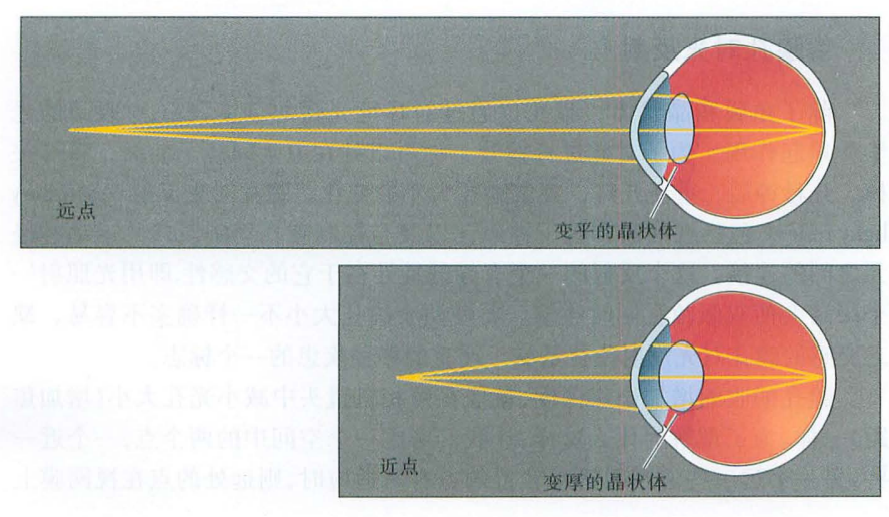
\includegraphics[height=0.3\textwidth]{img/pic3-2.png}
        \caption{适应性调节\label{pic3-2}}
    \end{figure}
\end{frame}

\subsection{视野}
\subsection{视锐度}

\begin{frame}
    \frametitle{视野}
    \begin{itemize}
        \item 眼睛的结构以及它在头部的位置使得特定时间内看到的外部世界收到限制。如图\ref{pic3-3},\textbf{视野}是指眼睛直视前方时视网膜所能看到的全部空间范围。值得注意的是,视野中的物体在视网膜上是反转的。
        \item 眼睛辨别两个相邻点的能力称为\textbf{视锐度}(visual acuity),主要取决于光感受器在视网膜上的分布和眼睛的折射精度。
        \item 视网膜上的距离可以用\textbf{视角}(visual angle)的度数来表示。当辨认视角为0.083°的字母时,视力为20/20
    \end{itemize}

    \begin{figure}
        \centering
        \subfigure[单眼视野\label{pic3-3}]{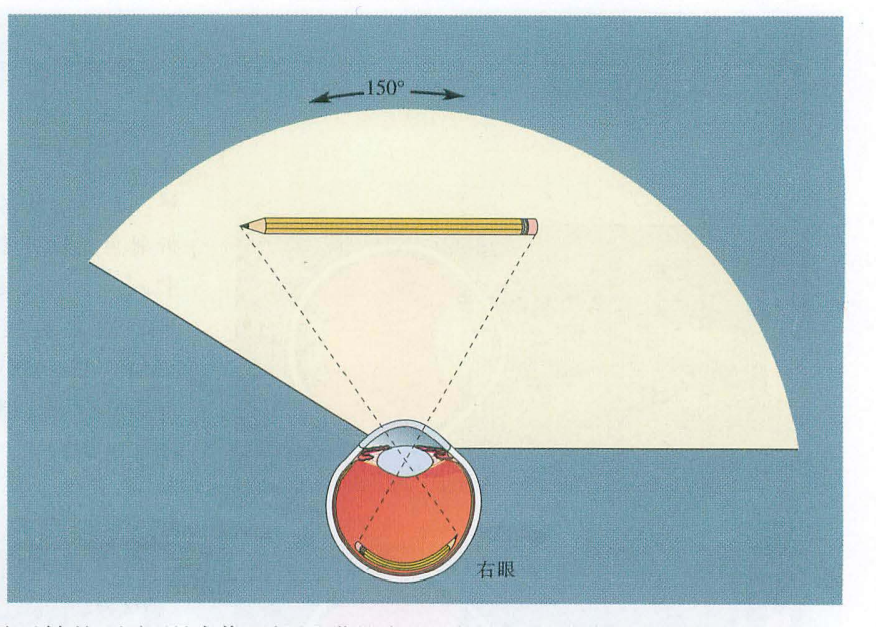
\includegraphics[height=0.3\textwidth]{img/pic3-3.png}}
        \subfigure[视角\label{pic3-4}]{ 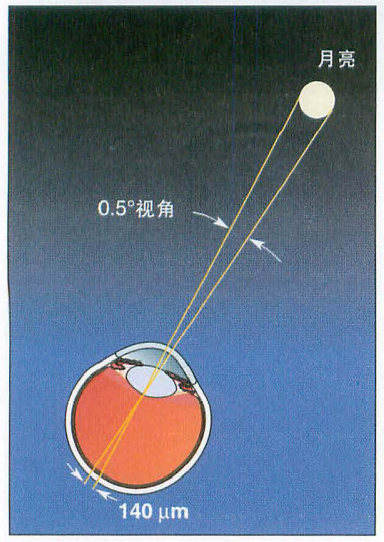
\includegraphics[height=0.3\textwidth]{img/pic3-4.png}}
    \end{figure}
\end{frame}
